\documentclass[border=10pt]{standalone}
\usepackage[svgnames]{xcolor}
\usepackage{amsmath}
\usepackage{pgfplots}
\pgfplotsset{compat=newest}
\usepackage[sfdefault]{FiraSans}
\usepackage{FiraMono}
\renewcommand*\familydefault{\sfdefault}
\begin{document}
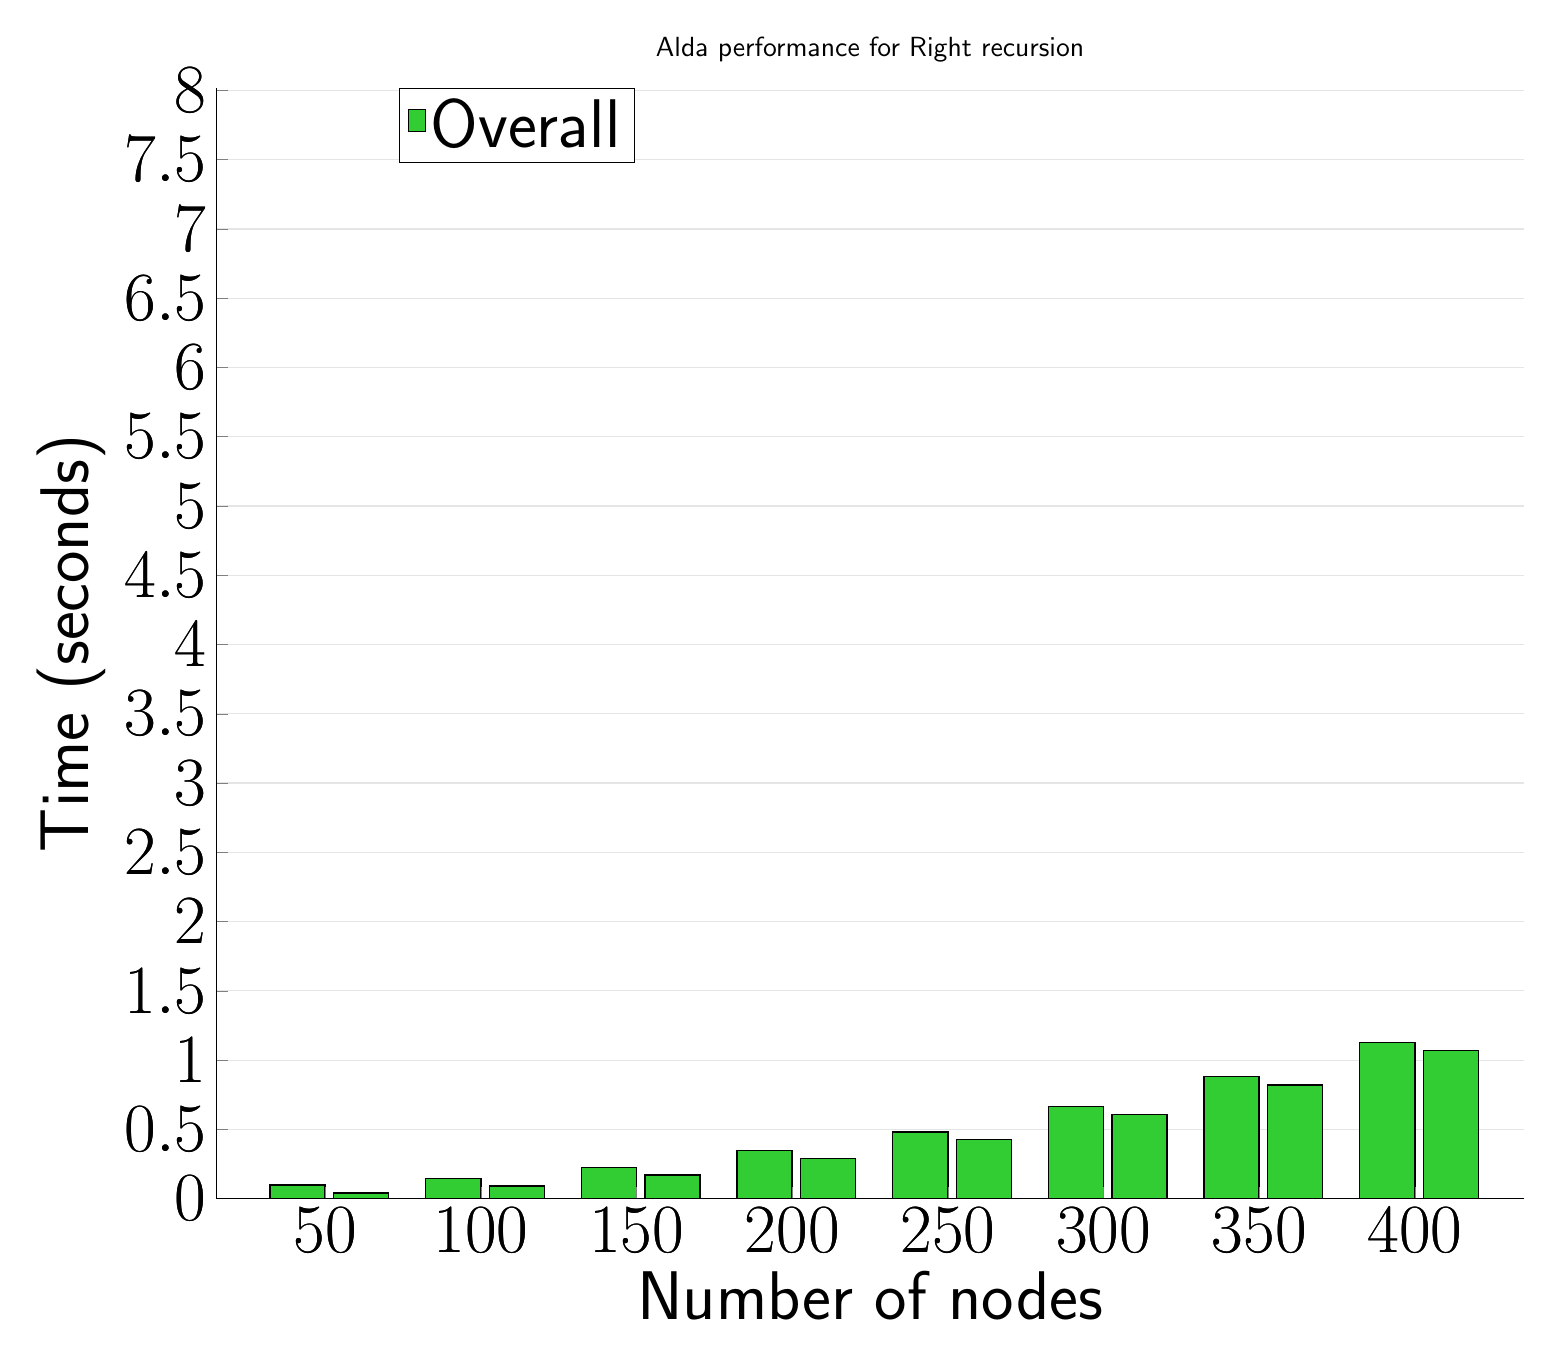
\begin{tikzpicture}
\begin{axis}[
   ybar stacked,
   title={Alda performance for Right recursion},
   bar shift=-10pt,
   width=1.5\textwidth,
   bar width=0.7cm,
   ymajorgrids, tick align=inside,
   major grid style={draw=gray!20},
   xtick=data,
   ymin=0, ymax=8.018999981880189,
   axis x line*=bottom,
   axis y line*=left,
   enlarge x limits=0.1,
   legend style={
       at={(0.23, 1)},
       anchor=north,
       legend columns=1,
       font=\Huge,
   },
   ylabel={Time (seconds)},
   xlabel={Number of nodes},
   label style={font=\Huge},
   tick label style={font=\Huge},
]
\addlegendimage{fill=LimeGreen, draw=black, line width=0.2pt}
\addlegendentry{Overall}
\addplot +[fill=LimeGreen, draw=black, line width=0.5pt] coordinates {
    (50, 0.09900000095367431)
    (100, 0.14700000286102294)
    (150, 0.2249999761581421)
    (200, 0.3459999799728394)
    (250, 0.4820000171661377)
    (300, 0.6659999847412109)
    (350, 0.8809999465942383)
    (400, 1.1289999723434447)
};
\end{axis}
\begin{axis}[
   ybar stacked,
   bar shift=13pt,
   width=1.5\textwidth,
   bar width=0.7cm,
   ymajorgrids, tick align=inside,
   major grid style={draw=none},
   xtick=data,
   ymin=0, ymax=8.018999981880189,
   axis x line*=none,
   axis y line*=none,
   enlarge x limits=0.1,
   label style={font=\Huge},
   tick label style={font=\Huge},
]
\addplot +[fill=LimeGreen, draw=black, line width=0.5pt] coordinates {
    (50, 0.040000000000000015)
    (100, 0.08999999999999998)
    (150, 0.16999999999999998)
    (200, 0.288)
    (250, 0.4250000000000001)
    (300, 0.608)
    (350, 0.8199999999999997)
    (400, 1.0670000000000002)
};
\end{axis}
\end{tikzpicture}

\end{document}
